\documentclass[nooutcomes]{ximera}
%% handout
%% space
%% newpage
%% numbers
%% nooutcomes


\newcommand{\RR}{\mathbb R}
\renewcommand{\d}{\,d}
\newcommand{\dd}[2][]{\frac{d #1}{d #2}}
\renewcommand{\l}{\ell}
\newcommand{\ddx}{\frac{d}{dx}}
\newcommand{\dfn}{\textbf}
\newcommand{\eval}[1]{\bigg[ #1 \bigg]}

\usepackage{multicol}

\renewenvironment{freeResponse}{
\ifhandout\setbox0\vbox\bgroup\else
\begin{trivlist}\item[\hskip \labelsep\bfseries Solution:\hspace{2ex}]
\fi}
{\ifhandout\egroup\else
\end{trivlist}
\fi} %% we can turn off input when making a master document

\title{Recitation \#7 - 3.1 Introducing the Derivative (Solutions)}  

\begin{document}
\begin{abstract}		\end{abstract}
\maketitle

\section*{Warm up:} 
Let $f(x) = x^{\frac{1}{3}}$.  Which of the following are true:
	
	\begin{enumerate}
	
	\item The graph of $f(x)$ has a tangent line at $x=0$.
	
	\item The derivative $f'(0)$ is defined.
	
	\end{enumerate}

		\begin{freeResponse}
		Below is a sketch of the graph for the function $f(x) = x^{\frac{1}{3}}$.  From this you can see that statement (a) is true but statement (b) is false.
			\begin{image}
			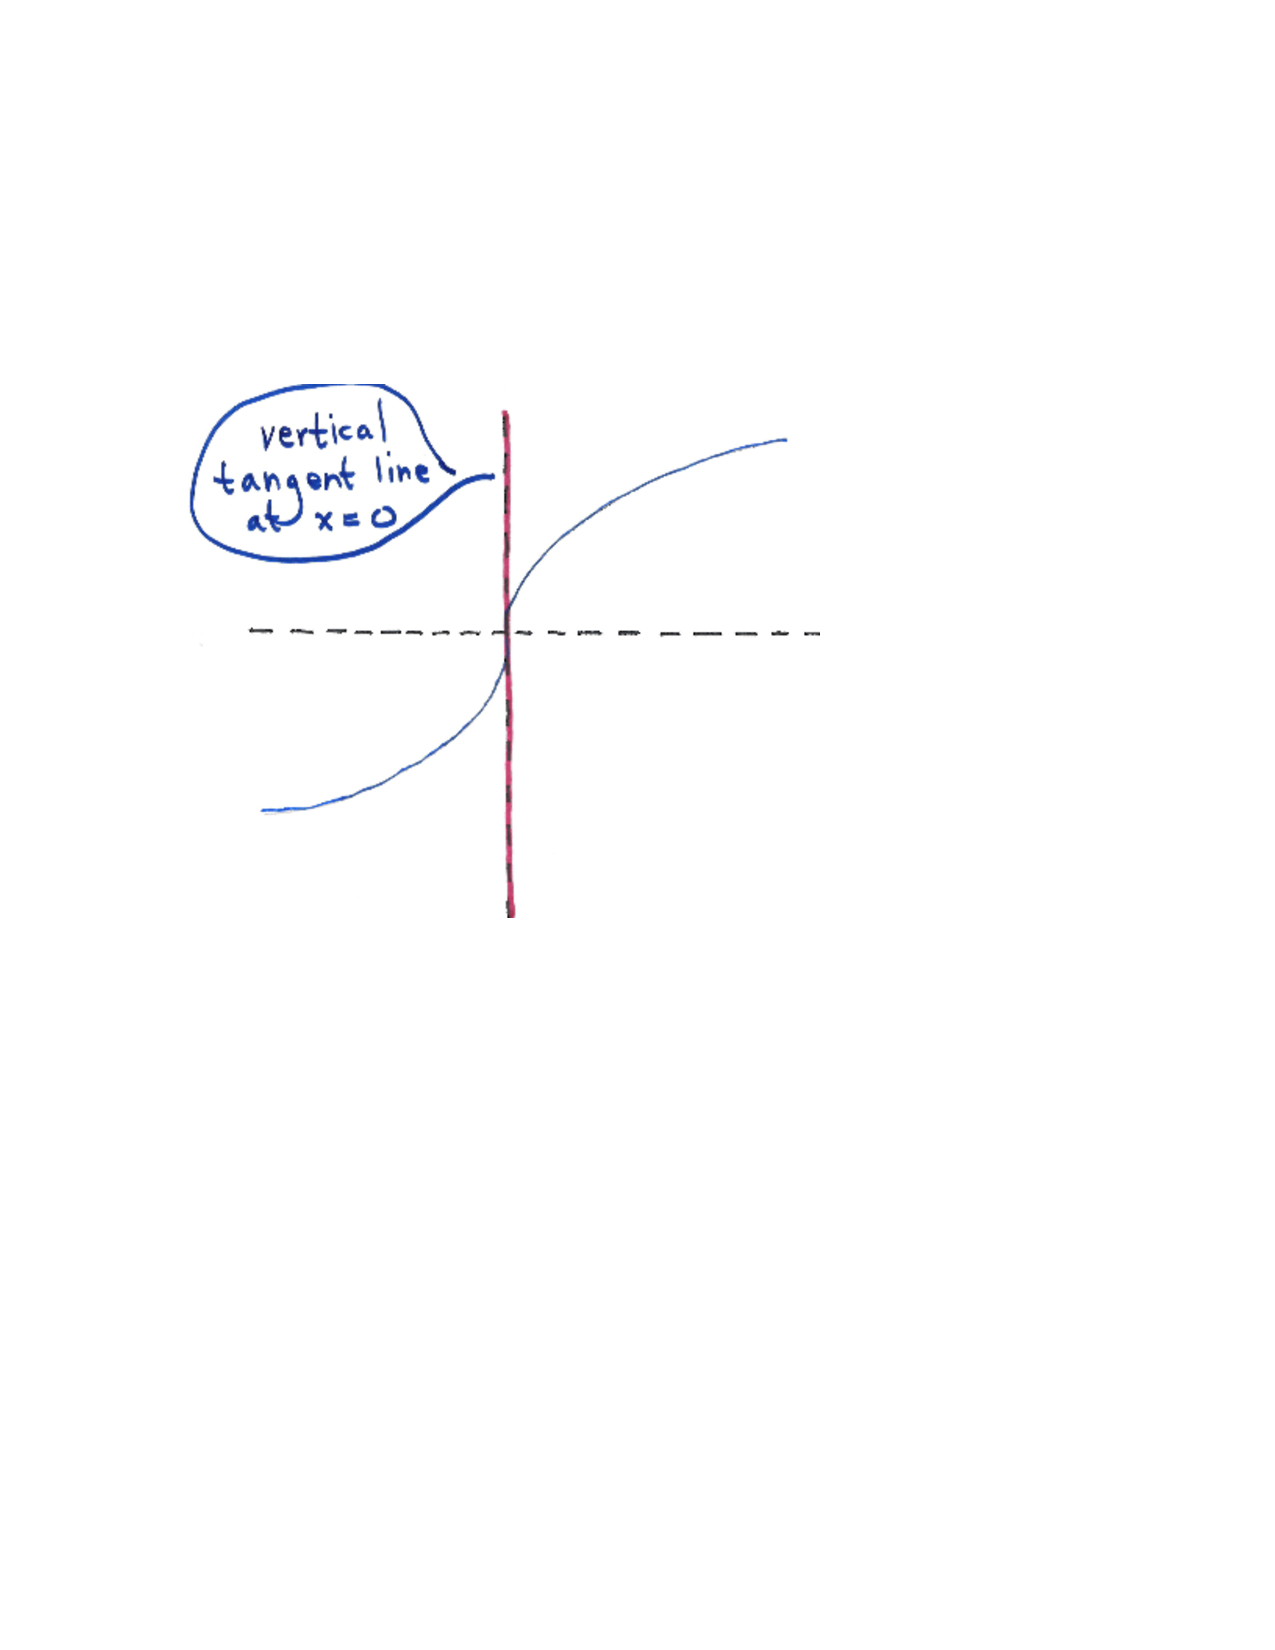
\includegraphics[trim= 170 350 250 180]{Figure1.pdf}
			\end{image}
		\end{freeResponse}
	
	

\section*{Group work:}

%problem 1
\begin{problem}
Discuss the similarities and differences between the two graphs below.  Why are the notations different?  Which are the secant lines?  Which are the tangent lines?  What are these graphes trying to communicate?

	$\begin{array}{lr}
		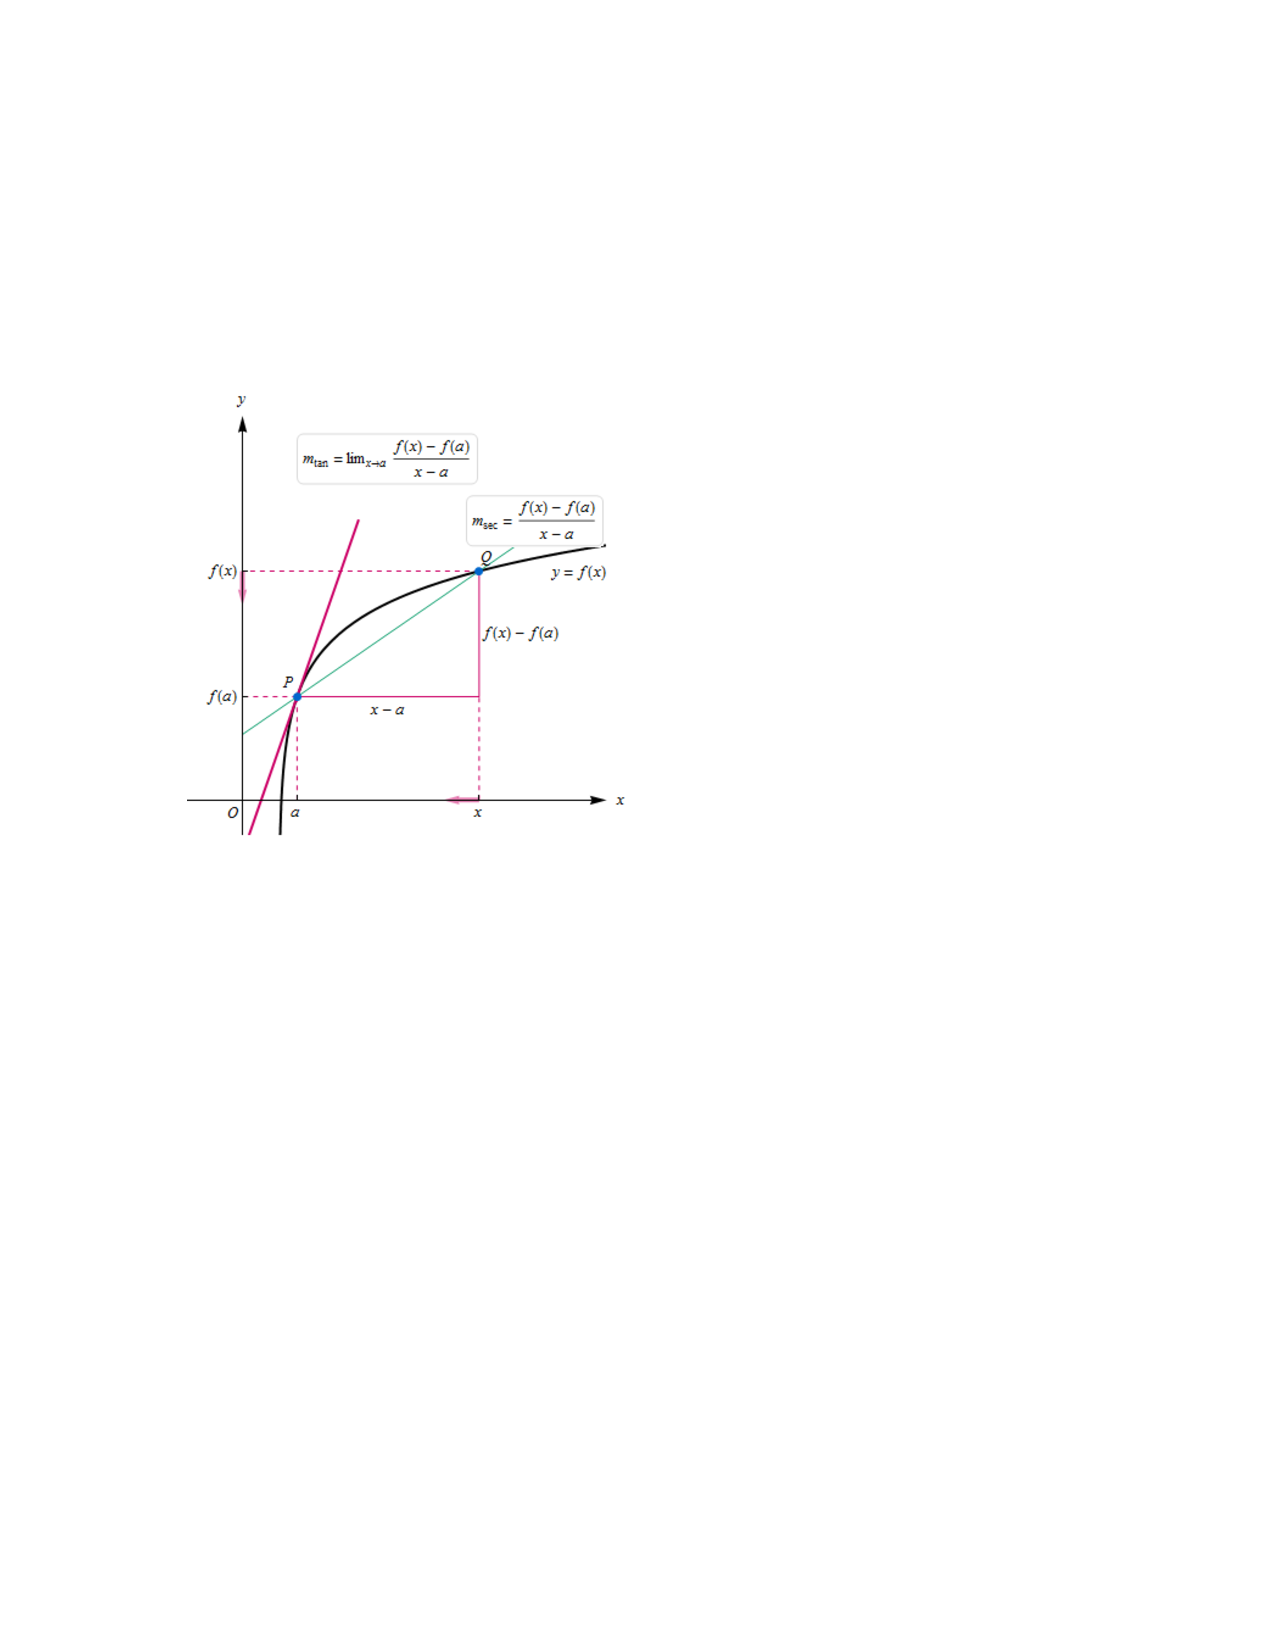
\includegraphics[trim= 150 350 250 180]{Figure2.pdf}
		&
		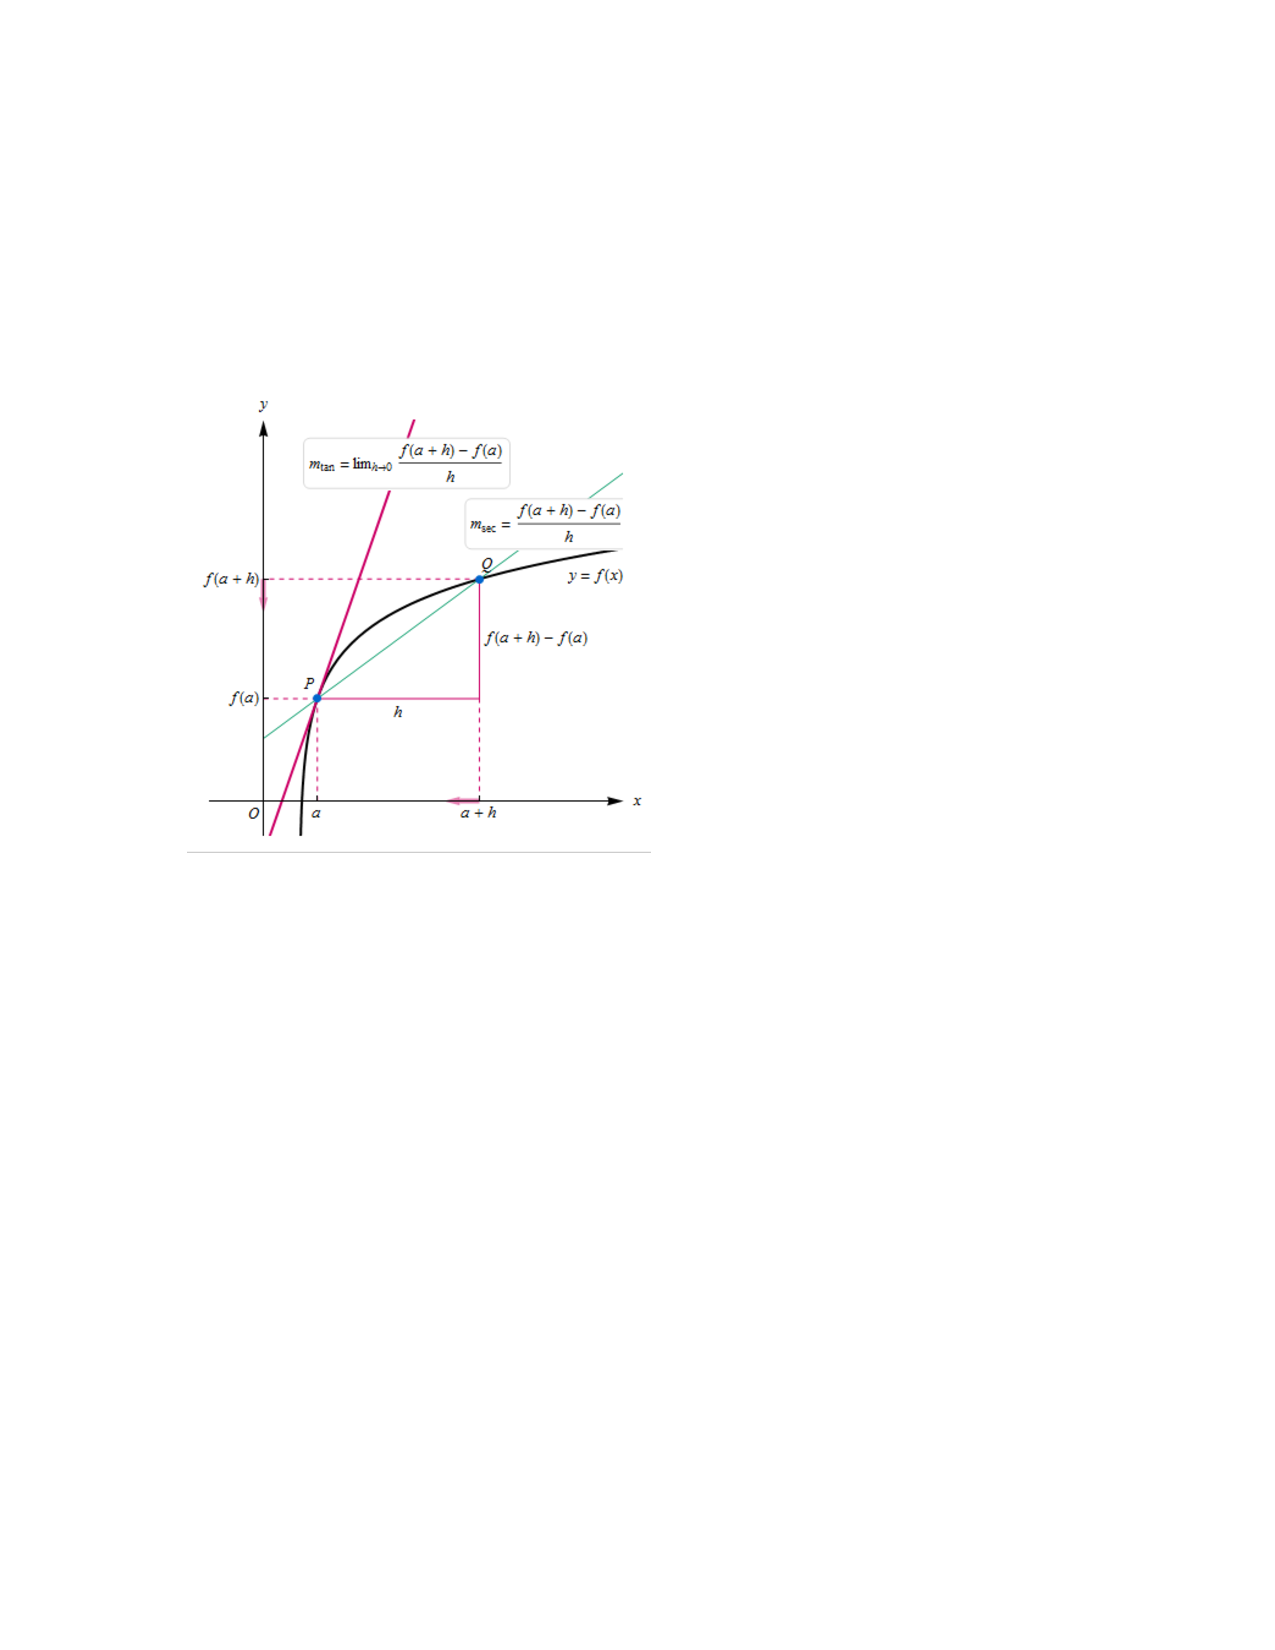
\includegraphics[trim= 140 350 250 180]{Figure3.pdf}
	\end{array}$

			\begin{freeResponse}
			The notations $\frac{f(x)-f(a)}{x-a}$ and $\frac{f(a+h)-f(a)}{h}$ both express the same number on the two graphs: they each give the slope of the secant line through $P$ 				and $Q$.  Note that $x-a=h$ and thus $x=a+h$.  Both notations are mathematically equivalent but in a given problem one may be easier to work with than the other.  

			Both graphs show that as we let $Q$ get closer to $P$, the secant line through $PQ$ approaches the tangent line through $P$.  We can summarize this by a suggestive 				phrase: the limit of the secant lines is the tangent line (it is suggestive but not precise).  Thus the limit of the slopes of the secant lines is the slope of the tangent line.
			\end{freeResponse}
\end{problem}
	
	
	
	
			
			

%problem 2			
\begin{problem}
Find the equation of the tangent line to the graph of the given function at $x=3$.

	\begin{enumerate}
	
	\item  $f(x) = -5x^2 + 7x - 9$
		\begin{freeResponse}
		For all three parts to problem 2, we first need to compute either $\lim_{h \to 0} \frac{f(3+h) - f(3)}{h}$ or $\lim_{x \to 3} \frac{f(x) - f(3)}{x-3}$ in order to compute the slope of the tangent line.  In problem 1 we saw that both formulas are mathematically equivalent, provided that the limits exist.  
		
		$\lim_{x \to 3} \frac{f(x) - f(3)}{x-3}
		= \lim_{x \to 3} \frac{(-5x^2 + 7x - 9) - (-45 + 21 - 9)}{x-3}
		= \lim_{x \to 3} \frac{-5x^2 + 7x - 9 + 33}{x-3}
		= \lim_{x \to 3} \frac{-5x^2 + 7x + 24}{x-3}
		= \lim_{x \to 3} \frac{(x-3)(-5x -8)}{x-3}
		= \lim_{x \to 3} (-5x - 8)
		= -5(3) - 8
		= -23.$
		
		Thus, the slope of the tangent line is $m_{tan}=-23$, and therefore the equation of the tangent line at $(3, f(3))$ is:
		
		$y - f(3) = -23(x-3)$
		
		$y + 33 = -23x + 69$
		
		$y = -23x + 36.$
		\end{freeResponse}
		
		
		
	
	\item  $f(x) = \sqrt{5x-4}$
		\begin{freeResponse}
		$m_{tan} = \lim_{h \to 0} \frac{f(3+h) - f(3)}{h}
		= \lim_{h \to 0} \frac{\sqrt{5(3+h) - 4} - \sqrt{11}}{h}.$
		
		At this step, we need to conjugate
		
		$m_{tan} = \lim_{h \to 0} \frac{\sqrt{5(3+h) - 4} - \sqrt{11}}{h} \cdot \frac{\sqrt{5(3+h) - 4} + \sqrt{11}}{\sqrt{5(3+h) - 4} + \sqrt{11}} 
		= \lim_{h \to 0} \frac{5(3+h) - 4 - 11}{h \left( \sqrt{5(3+h) - 4} + \sqrt{11} \right) }
		= \lim_{h \to 0} \frac{5h + 15 - 15}{h \left( \sqrt{5(3+h) - 4} + \sqrt{11} \right) }
		= \lim_{h \to 0} \frac{5}{\left( \sqrt{5(3+h) - 4} + \sqrt{11} \right) }
		= \frac{5}{\sqrt{5(3+0) - 4} + \sqrt{11}}
		= \frac{5}{2 \sqrt{11}}.$
		
		Thus, the slope of the tangent line is $m_{tan}=\frac{5}{2\sqrt{11}}$, and therefore the equation of the tangent line at $(3, f(3))$ is:
		
		$y - f(3) = \frac{5}{2\sqrt{11}}(x-3)$
		
		$y - \sqrt{11} = \frac{5}{2\sqrt{11}}(x - 3).$
		\end{freeResponse}
		
	
	\item  $f(x) = \frac{x}{x-5}$
		\begin{freeResponse}
		$m_{tan} = \lim_{x \to 3} \frac{f(x) - f(3)}{x-3}
		= \lim_{x \to 3} \frac{\frac{x}{x-5} - \frac{3}{3-5}}{x-3}
		= \lim_{x \to 3} \frac{\frac{x}{x-5} + \frac{3}{2}}{x-3}
		= \lim_{x \to 3} \frac{\frac{2x}{2(x-5)} + \frac{3(x-5)}{2(x-5)}}{x-3}
		= \lim_{x \to 3} \frac{\frac{2x + 3x - 15}{2(x-5)}}{x-3}
		= \lim_{x \to 3} \frac{5x-15}{2(x-5)} \cdot \frac{1}{x-3}$
		
		$= \lim_{x \to 3} \frac{5(x-3)}{2(x-5)} \cdot \frac{1}{x-3}
		= \lim_{x \to 3} \frac{5}{2(x-5)}
		= \frac{5}{2(3-5)} = -\frac{5}{4}.$
		
		Thus, the slope of the tangent line is $m_{tan}=- \frac{5}{4}$, and therefore the equation of the tangent line at $(3, f(3))$ is:
		
		$y - f(3) = - \frac{5}{4}(x-3)$
		
		$y + \frac{3}{2} = - \frac{5}{4}x + \frac{15}{4}$
		
		$y = - \frac{5}{4} x + \frac{9}{4}.$
		\end{freeResponse}
		
	
	\end{enumerate}
\end{problem}









%problem 3			
\begin{problem}
Let $f(x) = |5-x|$.
	
	\begin{enumerate}
	
	%part a
	\item For $a < 5$, find $f'(a)$.
	
		\begin{freeResponse}
		Recall that $f'(a) = \lim_{x \to a} \frac{f(x) - f(a)}{x-a}$.  When $a < 5$, $0 < 5-a$ and so $f(a) = |5-a| = 5-a$.  Since we are considering the limit as $x$ approaches $a$, we may also assume that $x > 5$ and therefore $f(x) = 5-x$.  Thus
		
		$f'(a) = \lim_{x \to a} \frac{f(x) - f(a)}{x-a}
		= \lim_{x \to a} \frac{(5-x) - (5-a)}{x-a}
		= \lim_{x \to a} \frac{-(x-a)}{x-a}
		= \lim_{x \to a} -1 = -1$.
		\end{freeResponse}
		
		
	
	%part b
	\item For $a > 5$, find $f'(a)$.
	
		\begin{freeResponse}
		When $a > 5$, $0 > 5-a$ and so $f(a) = |5-a| = -(5-a) = a-5$.  Since we are considering the limit as $x$ approaches $a$, we may also assume that $x < 5$ and therefore $f(x) = x-5$.  Thus
		
		$f'(a) = \lim_{x \to a} \frac{f(x) - f(a)}{x-a}
		= \lim_{x \to a} \frac{(x-5) - (a-5)}{x-a}
		= \lim_{x \to a} \frac{x-a}{x-a}
		= \lim_{x \to a} 1 = 1$.

		\end{freeResponse}
		
		
	
	%part c
	\item Use your work from parts (a) and (b) to answer the question ``Does $f'(5)$ exist and, if so, what is $f'(a)$?".
	
		\begin{freeResponse}
		$f'(5) = \lim_{x \to 5} \frac{f(x) - f(5)}{x-5}$ provided this limit exists.  We know from part (a) that, as $x$ approaches $5$ from the left, this limit exists and equals $-1$.  We similarly know from part (b) that, as $x$ approaches $5$ from the right, this limit exists and equals $1$.  Since $\lim_{x \to 5^-} \frac{f(x) - f(5)}{x-5} = -1 \neq 1 = \lim_{x \to 5^+} \frac{f(x) - f(5)}{x-5}$, we know that $\lim_{x \to 5} \frac{f(x) - f(5)}{x-5}$ DNE.  Therefore, $f'(5)$ does not exist.
		\end{freeResponse}
		
		
	
	\end{enumerate}


\end{problem}
	
	
	
	
	
	
	
	
	

	










								
				
				
	














\end{document} 


















